\documentclass{article}
\usepackage{tikz}
\usepackage{amsmath}
\usepackage[margin=1in]{geometry}
\title{%Reversing Gumbo for SysMLv2 Compatibility in IR-Based Code Generation}%
Compositional Model Translation for IR-Based Code Generation: From SysMLv2 to IR through Gumbo}
\author{Amer Tahat \and Isaac Amundson}
\date{}

\begin{document}

\maketitle

\section*{Abstract}
This document presents a compositional translation pipeline for IR-based code generation that bridges high-level system models in SysMLv2 with a KS Gumbo-based backend. A reverse transformation from SysMLv2 to Gumbo enables reuse of the existing Serum toolchain, which maps Gumbo specifications to an Intermediate Representation (IR) for code synthesis. The transformation chain is visualized to show how IR can be generated from SysMLv2 via composition of functions.

\section*{Mapping Overview}
Let $X$ be a specification written in Gumbo. The KS tool-chain defines a transformation $\mathrm{T}_{\mathrm{KS}}$ such that:
\begin{equation*}
    \mathrm{T}_{\mathrm{KS}}(X) \in \text{IR}
\end{equation*}

We define a reverse transformation $\mathrm{T}^{-1}_{\mathrm{COL}}$ from Gumbo to SysMLv2, created by the Collins team:
\begin{equation*}
    \mathrm{T}^{-1}_{\mathrm{COL}}(X) = Y \in \text{SysMLv2}
\end{equation*}

To reuse the Serum backend, we define a composition of functions:
\begin{equation*}
    \text{IR}(Y) = \left( \mathrm{T}_{\mathrm{KS}} \circ \mathrm{T}_{\mathrm{COL}} \right)(Y)
\end{equation*}

\section*{Pipeline Diagram}

\begin{center}
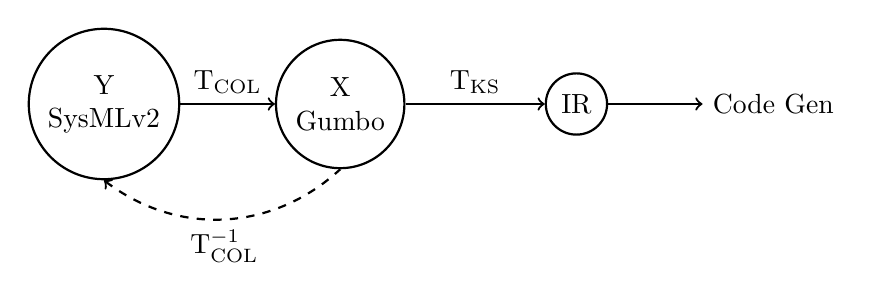
\begin{tikzpicture}[->, thick, node distance=3cm, align=center]
  \node (sysml) [circle, draw] {Y \\ SysMLv2};
  \node (gumbo) [circle, draw, right of=sysml] {X \\ Gumbo};
  \node (ir) [circle, draw, right of=gumbo] {IR};
  \node (cg) [right of=ir, node distance=2.5cm] {Code Gen};

  % Forward arrows
  \draw (sysml) -- node[above] {$\mathrm{T}_{\mathrm{COL}}$} (gumbo);
  \draw (gumbo) -- node[above] {$\mathrm{T}_{\mathrm{KS}}$} (ir);
  \draw (ir) -- (cg);

  % Reverse arrow below, curved and labeled underneath
  \draw[dashed, <-, thick] (sysml.south) to[bend right=40] node[below] {$\mathrm{T}^{-1}_{\mathrm{COL}}$} (gumbo.south);
\end{tikzpicture}
\end{center}

\section*{Conclusion}
This approach enables seamless reuse of the KS backend by mapping SysMLv2 specifications into the Gumbo domain, and then proceeding with the original IR generation pipeline.

\end{document}